\section{Game Design}

% Base on our pilot study results, we understand that if the cooperative game require High-Level Feature Communication, play it with non-common language player is really frustrating. According to GameFlow[1], games challenging should match the player’s skill level, If the challenges are greater than the skills, the result is anxiety and frustrating, if the challenges are less than the skills, the result is apathy and boring.

Based on our pilot study results, we realize that if playing cooperative games requires high-level-feature communication, playing with non-common language players would feel deeply frustrated. According to GameFlow\cite{GD1}, game challenges should match the player's skill level. If the challenges are greater than the player's skills, the gameplay result will be anxiety and frustrating. But, by constrast, if the challenges are less than the player's skills, the result will be apathy and boring.

% According to our observation, play cooperative game with different language speaker will significantly decrease cooperative skills which is really important for most cooperative games and the game challenge become too hard for this situation and causing frustrating. The most easy way to solve this problem is to decrease the game challenge difficulty for non-common language players, but it is not practical for commercial games because the players with common language would feel boring with no difficulty.

According to our observation, playing cooperative game with different language speaker will significantly decrease cooperative skills which is really important for most cooperative games. And game challenges would become too hard for this situation and cause frustrated. The easiest way to solve this problem is to decrease the game's difficulty for non-common language players. Nevertheless, this method is not practical for commercial games because it will make players with common language feel boring with no difficulty while playing the game (see Figure~\ref{fig:GD_F1}).  

\begin{figure}[!h]
\centering
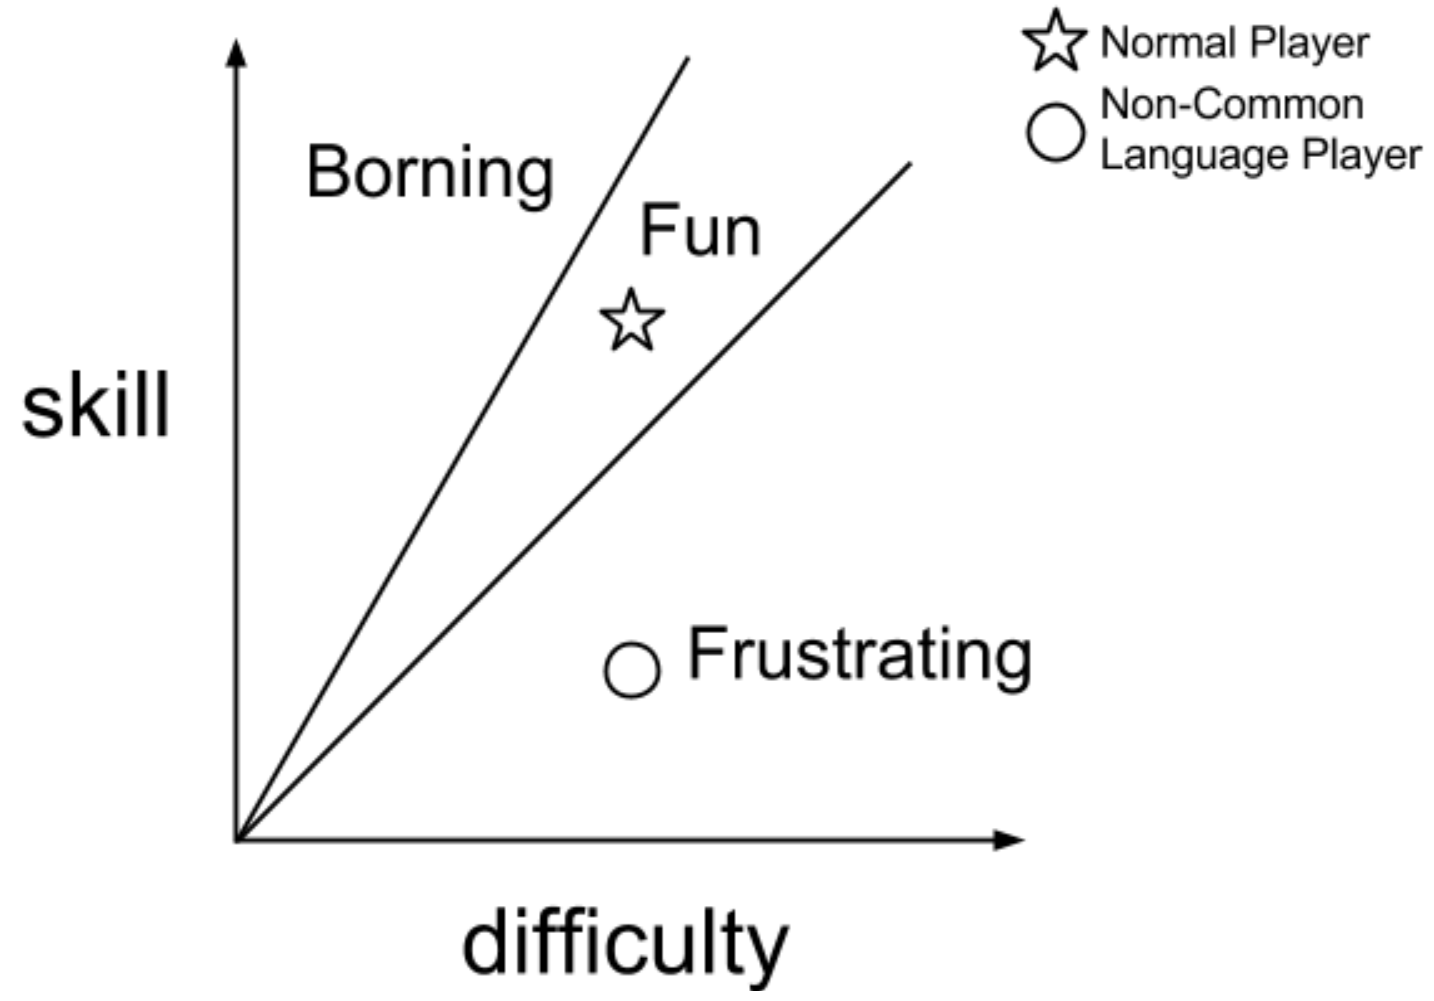
\includegraphics[width=0.9\columnwidth]{Figures/GD_F1.png}
\caption{Language boundary is causing player's skill difference}
\label{fig:GD_F1}
\end{figure}

\subsection{Body Language}

% Human communication involves not only speech, but also a wide variety of gestures and body motions. Body language is the most effective means of communicating un-spoken emotions, a non-verbal way to impart your thoughts without verbalizing it. According to The 7\% Rule [1], communication is only 7 percent verbal and 93 percent non-verbal. The non-verbal component was made up of body language(55 percent) and tone of voice (38 percent).

Consist of human communication, there are not only speech but also inclusive of various gestures and body motions. Body language, a non-verbal way to transmit your thoughts without verbalizing. Accouring to the 7\% Rule\cite{GD2}, the influence for communication for verbal is only 7\% but is 93\% for non-verbal expression. And the non-varbal expression is made up of body language (55\%) and tones of voice (38\%).

% Charades[2] is a word guessing game.In the form most played today, it is an acting game in which one player acts out a word or phrase, often by miming similar sounding words, and the other players guess the word or phrase. The idea is to use physical rather than verbal language to convey the meaning to another party.

Charades\cite{GD3} is a word guessing game. Charades is an acting game in which one player acts as a word or a phrase, and sometime imitates a similar pronounced words, while the other players guess for the answer. The main idea is to use body to make physical expression rather than using verbal language. 

% Inspired by The 7\% Rule and Charades, We suggest to use body language as a communication manner in cooperative game to normalize player’s communication skill, so that no matter players are playing with different language speaker or not, their communication skill is near enough for game developer to design a proper difficulty to please players.

Inspired by the 7\% Rule and the Charades, we suggested to use body language as a communicate manner in cooperative game to normalize player's communication skill. With this idea, whether players are playing with different language speakers or not, their communication skill is near enough for game developer to design a proper difficulty to increase players' enjoyment.


\subsection{Prototype-Mute Robot}

% To explore our idea that using body language communication in cooperative game , we have designed Mute Robot, a game in which 2 players must cooperate to solve a series of puzzle challenges by communicating through body language only.

The main idea we want to explore is the influence of using body language in cooperative game. In order to find out the answer, we had designed Mute Robot, a game in which 2 players must cooperate to solve a series of puzzle challenges by communicating through body language only.

To encourage players to use body language, we have designed an asymmetric puzzle system, with only one player receiving puzzle hints. The player will use body language to guide the other player to solve the puzzle. Taking one of our game stage as an example (see Figure~\ref{fig:GD_F2}), there is a locked door on the right side which obstructs both players’ route to the next stage. The top player can’t see the puzzle-solving hints but can turn the wheel to the match the puzzle answer, which consequently opens the locked door. The only way to pass the stage is for the bottom player to convey the puzzle-solving messages to the other player with body language.

\begin{figure}[!h]
\centering
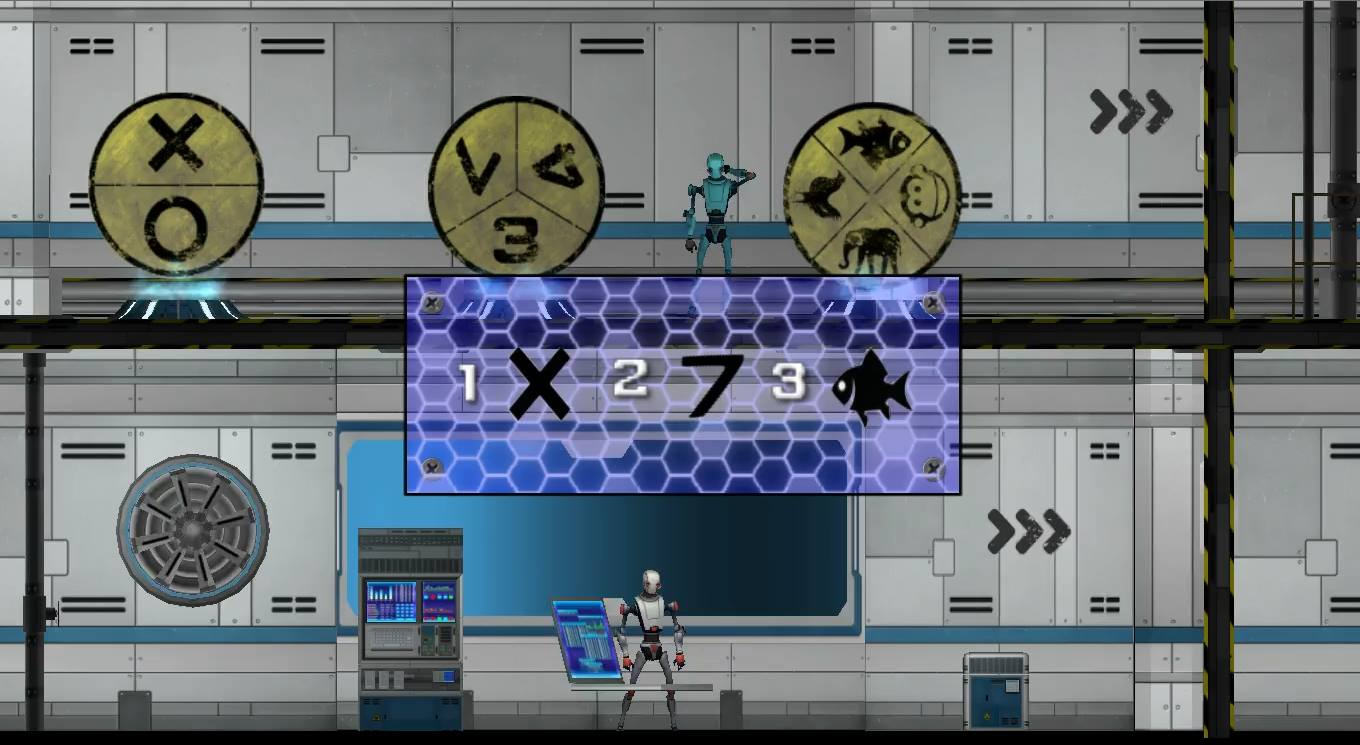
\includegraphics[width=0.9\columnwidth]{Figures/GD_F2.jpg}
\caption{The asymmetric puzzle game design in one of Mute Robot’s stages.}
\label{fig:GD_F2}
\end{figure}
hi

\subsection{Level Design}
hi
\subsection{System Implementation}
hi